\makeatletter

\usetikzlibrary{arrows}
\usetikzlibrary{scopes}

\pgfdeclareshape{boiler}
{
	\savedanchor{\center}{\pgfpointorigin}
	\savedanchor{\boxsw}{\pgfpoint{-.5cm}{-.5cm}}
	\savedanchor{\boxne}{\pgfpoint{.5cm}{.5cm}}
	\savedanchor{\boxn}{\pgfpoint{0cm}{.5cm}}
	\savedanchor{\ziga}{\pgfpoint{.25cm}{.75cm}}
	\savedanchor{\zigb}{\pgfpoint{-.25cm}{.75cm}}
	\savedanchor{\zigc}{\pgfpoint{0cm}{1cm}}

	\anchor{center}{\center}
	\anchor{text}{
		\pgf@x=-.5\wd\pgfnodeparttextbox
		\pgf@y=-.5\ht\pgfnodeparttextbox
	}
	\anchor{s}{\pgfpoint{0cm}{-.5cm}}
	\anchor{n}{\pgfpoint{0cm}{1cm}}

	\backgroundpath{
		\pgfpathrectanglecorners{\boxsw}{\boxne}

		\pgfpathmoveto{\boxn}
		\pgfpathlineto{\ziga}
		\pgfpathlineto{\zigb}
		\pgfpathlineto{\zigc}
		\pgfusepath{stroke}
	}
}

\pgfdeclareshape{turbine}
{
	\savedanchor{\center}{\pgfpointorigin}
	\savedanchor{\sw}{\pgfpoint{-.75cm}{-.33cm}}
	\savedanchor{\nw}{\pgfpoint{-.75cm}{.33cm}}
	\savedanchor{\se}{\pgfpoint{.75cm}{-.75cm}}
	\savedanchor{\ne}{\pgfpoint{.75cm}{.75cm}}

	\anchor{center}{\center}
	\anchor{text}{
		\pgf@x=-.5\wd\pgfnodeparttextbox
		\pgf@y=-.5\ht\pgfnodeparttextbox
	}
	\anchor{nw}{\nw}
	\anchor{se}{\se}
	\anchor{sw}{\sw}

	\backgroundpath{
		\pgfpathmoveto{\nw}
		\pgfpathlineto{\ne}
		\pgfpathlineto{\se}
		\pgfpathlineto{\sw}
		\pgfpathclose
		\pgfusepath{stroke}
	}
}

\pgfdeclareshape{condenser}
{
	\savedanchor{\center}{\pgfpointorigin}
	\savedanchor{\s}{\pgfpoint{0cm}{-.5cm}}
	\savedanchor{\n}{\pgfpoint{0cm}{.5cm}}
	\savedanchor{\ne}{\pgfpoint{.75cm}{.35cm}}
	\savedanchor{\se}{\pgfpoint{.75cm}{-.35cm}}
	\savedanchor{\nx}{\pgfpoint{.25cm}{.35cm}}
	\savedanchor{\sx}{\pgfpoint{.25cm}{-.35cm}}
	\savedanchor{\mnx}{\pgfpoint{-.25cm}{.175cm}}
	\savedanchor{\msx}{\pgfpoint{-.25cm}{-.175cm}}
	\savedanchor{\mx}{\pgfpoint{.25cm}{0cm}}

	\anchor{center}{\center}
	\anchor{text}{
		\pgf@x=.66cm
		\pgf@y=-.5\ht\pgfnodeparttextbox
	}
	\anchor{n}{\n}
	\anchor{s}{\s}
	\anchor{ne}{\ne}
	\anchor{se}{\se}

	\backgroundpath{
		\pgfpathcircle{\center}{.5cm}

		\pgfpathmoveto{\ne}
		\pgfpathlineto{\nx}
		\pgfpathlineto{\mnx}
		\pgfpathlineto{\mx}
		\pgfpathlineto{\msx}
		\pgfpathlineto{\sx}
		\pgfpathlineto{\se}
		\pgfusepath{stroke}
	}
}

\pgfdeclareshape{pump}
{
	\savedanchor{\center}{\pgfpointorigin}
	\savedanchor{\w}{\pgfpoint{-.33cm}{0cm}}
	\savedanchor{\e}{\pgfpoint{.33cm}{0cm}}
	\savedanchor{\arrw}{\pgfpoint{-.25cm}{0cm}}
	\savedanchor{\arre}{\pgfpoint{.25cm}{0cm}}
	\savedanchor{\arrne}{\pgfpoint{.1cm}{.066cm}}
	\savedanchor{\arrse}{\pgfpoint{.1cm}{-.066cm}}

	\anchor{center}{\center}
	\anchor{text}{
		\pgf@x=-.5\wd\pgfnodeparttextbox
		\pgf@y=.15cm
		\advance \pgf@y by \ht\pgfnodeparttextbox
	}
	\anchor{w}{\w}
	\anchor{e}{\e}

	\backgroundpath{
		\pgfpathcircle{\center}{.33cm}

		\pgfpathmoveto{\arrw}
		\pgfpathlineto{\arre}
		\pgfusepath{stroke}

		\pgfpathmoveto{\arre}
		\pgfpathlineto{\arrne}
		\pgfpathlineto{\arrse}
		\pgfpathclose
		\pgfusepath{fill}
	}
}

\pgfdeclareshape{pumpl}
{
	\savedanchor{\center}{\pgfpointorigin}
	\savedanchor{\w}{\pgfpoint{-.33cm}{0cm}}
	\savedanchor{\e}{\pgfpoint{.33cm}{0cm}}
	\savedanchor{\arrw}{\pgfpoint{-.25cm}{0cm}}
	\savedanchor{\arre}{\pgfpoint{.25cm}{0cm}}
	\savedanchor{\arrnw}{\pgfpoint{-.1cm}{.066cm}}
	\savedanchor{\arrsw}{\pgfpoint{-.1cm}{-.066cm}}

	\anchor{center}{\center}
	\anchor{text}{
		\pgf@x=-.5\wd\pgfnodeparttextbox
		\pgf@y=.15cm
		\advance \pgf@y by \ht\pgfnodeparttextbox
	}
	\anchor{e}{\e}
	\anchor{w}{\w}

	\backgroundpath{
		\pgfpathcircle{\center}{.33cm}

		\pgfpathmoveto{\arre}
		\pgfpathlineto{\arrw}
		\pgfusepath{stroke}

		\pgfpathmoveto{\arrw}
		\pgfpathlineto{\arrnw}
		\pgfpathlineto{\arrsw}
		\pgfpathclose
		\pgfusepath{fill}
	}
}

\pgfdeclareshape{heatxchg}
{
	\savedanchor{\center}{\pgfpointorigin}
	\savedanchor{\sw}{\pgfpoint{-.5cm}{-.5cm}}
	\savedanchor{\ne}{\pgfpoint{.5cm}{.5cm}}

	\savedanchor{\w}{\pgfpoint{-.5cm}{0cm}}
	\savedanchor{\e}{\pgfpoint{.5cm}{0cm}}
	\savedanchor{\zw}{\pgfpoint{-.3cm}{0cm}}
	\savedanchor{\ze}{\pgfpoint{.3cm}{0cm}}
	\savedanchor{\zn}{\pgfpoint{0cm}{.4cm}}
	\savedanchor{\zs}{\pgfpoint{0cm}{-.4cm}}

	\anchor{center}{\center}
	\anchor{text}{
		\pgf@x=.45cm
		\pgf@y=.4cm
		\advance \pgf@x by -\wd\pgfnodeparttextbox
		\advance \pgf@y by -\ht\pgfnodeparttextbox
	}
	\anchor{e}{\e}
	\anchor{w}{\w}
	\anchor{n}{\pgfpoint{0cm}{.5cm}}
	\anchor{s}{\pgfpoint{0cm}{-.5cm}}

	\backgroundpath{
		\pgfpathrectanglecorners{\sw}{\ne}

		\pgfpathmoveto{\e}
		\pgfpathlineto{\ze}
		\pgfpathlineto{\zs}
		\pgfpathlineto{\zn}
		\pgfpathlineto{\zw}
		\pgfpathlineto{\w}
		\pgfusepath{stroke}
	}
}

\pgfdeclareshape{heatnode}
{
	\savedanchor{\center}{\pgfpointorigin}

	\anchor{center}{\center}

	\backgroundpath{
		\pgfpathcircle{\center}{.5mm}
		\pgfusepath{fill}
	}
}

\makeatother

\begin{figure}
	\label{graf-przyklad}

	\subfloat[graf-przyklad-sch][Schemat cieplny]{
		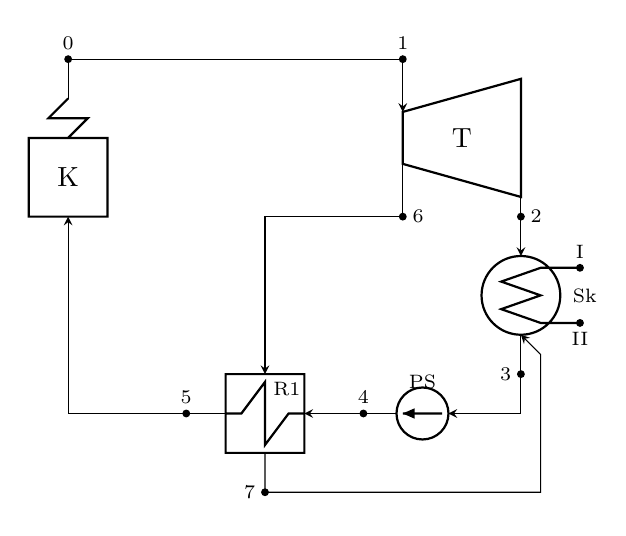
\begin{tikzpicture}
			{ [thick]
				\node[boiler] (K) at (0,3.5) {K};
				\node[turbine] (T) at (5,4) {T};
				\node[condenser, font=\scriptsize] (S) at (5.75,2) {Sk};
				\node[pumpl, font=\scriptsize] (PS) at (4.5,.5) {PS};
				\node[heatxchg, font=\scriptsize] (R1) at (2.5,.5) {R1};
			}

			{ [font=\scriptsize]
				\node[heatnode] (P0) at (0,5) {};
				\node[above] at (P0) {0};
				\node[heatnode] (P1) at (4.25,5) {};
				\node[above] at (P1) {1};
				\node[heatnode] (P2) at (5.75,3) {};
				\node[right] at (P2) {2};
				\node[heatnode] (P3) at (5.75,1) {};
				\node[left] at (P3) {3};
				\node[heatnode] (P4) at (3.75,.5) {};
				\node[above] at (P4) {4};
				\node[heatnode] (P5) at (1.5,.5) {};
				\node[above] at (P5) {5};
				\node[heatnode] (P6) at (4.25,3) {};
				\node[right] at (P6) {6};
				\node[heatnode] (P7) at (2.5,-.5) {};
				\node[left] at (P7) {7};
				\node[heatnode] (Pi) at (6.5,2.35) {};
				\node[above] at (Pi) {I};
				\node[heatnode] (Pii) at (6.5,1.65) {};
				\node[below] at (Pii) {II};
			}

			{ [-stealth]
				\draw (K.n) |- (2,5) -| (T.nw);
				\draw (T.se) -- (S.n);
				\draw (S.s) |- (PS.e);
				\draw (PS.w) -- (R1.e);
				\draw (R1.w) -| (K.s);

				\draw (T.sw) |- (3,3) -| (R1.n);
				\draw (R1.s) |- (6,-.5) -- ++(0,1.75) -- (S.s);
			}
		\end{tikzpicture}
	}%
%
	\subfloat[graf-przyklad-w1][Wariant A]{
		\begin{tikzpicture}
			{ [font=\scriptsize]
				\node[heatnode] (P0) at (1.5,5) {};
				\node[above] at (P0) {0};
				\node[heatnode] (P1) at (4.25,5) {};
				\node[above] at (P1) {1};
				\node[heatnode] (P2) at (5.75,3) {};
				\node[above] at (P2) {2};
				\node[heatnode] (P3k) at (5.75,.5) {};
				\node[heatnode] (P3) at (5,0) {};
				\node[below] at (P3) {3};
				\node[heatnode] (P4) at (3.75,.5) {};
				\node[left] at (P4) {4};
				\node[heatnode] (P5) at (3.75,3) {};
				\node[above] at (P5) {5};
				\node[heatnode] (P6) at (4.25,3) {};
				\node[above right] at (P6) {6};
				\node[heatnode] (P7) at (4.25,.5) {};
				\node[above right] at (P7) {7};
				\node[heatnode] (Pi) at (6.25,3) {};
				\node[above] at (Pi) {I};
				\node[heatnode] (Pii) at (6.25,.5) {};
				\node[below] at (Pii) {II};
			}

			{ [-stealth, shorten >=1mm, shorten <=1mm, font=\scriptsize]
				\draw (P0) -- (P1) node[above, pos=.5] {(rurociąg)};
				\draw (P1) -- (P6);
				\draw (P6) -- (P2);
				\draw (P2) -- (P3k);
				\draw (P3k) -- (P3);
				\draw (P3) -| (P4) node[below right, pos=.5] {(PS)};
				\draw (P4) -- (P5);
				\draw (P5) -| (P0) node[above right, pos=.5] {(K)};
				\draw (P6) -- (P7);
				\draw (P7) -- (P3);
				\draw (Pii) -- (Pi);
			}

			{ [color=red, dashdotted, font=\scriptsize]
				\draw (P6) +(-.1,-.1) rectangle (5.85,5.1)
					node[below left] {(T)};
				\draw (P4) +(-.1,-.1) rectangle (4.35,3.1);
				\draw (P3k) +(-.1,-.1) rectangle (6.35,3.1);
				\draw (P7) +(-.1,.1) rectangle (5.85,-.1);
				\path (P7) -- (P3k) node[pos=.5] {(miesz.)};
			}

			{ [color=blue, -stealth, shorten >=1mm, shorten <=1mm, font=\scriptsize]
				\draw (P7) ++(0,1) -- ++(-.5,0);
				\draw (P7) ++(0,1.25) -- ++(-.5,0);
				\draw (P7) ++(0,1.5) -- ++(-.5,0)
					node[above, pos=.5, color=red] {R1};
				\draw (P3k) ++(0,1) -- ++(.5,0);
				\draw (P3k) ++(0,1.25) -- ++(.5,0);
				\draw (P3k) ++(0,1.5) -- ++(.5,0)
					node[above, pos=.5, color=red] {Sk};
			}
		\end{tikzpicture}
	}

	\caption{Reprezentacja przykładowego obiegu cieplnego za~pomocą teorii grafów}
\end{figure}
